
\chapter{Sensae Console Domains}
\label{appendix:design:domain:bounded_contexts}

The \textbf{Bounded Context} concept, defined by \cite{evans2014domain}, refers to an unified model - with well-defined boundaries and internally consistent - that is, a single piece in a larger system composed by various bounded contexts.

The concept \textbf{Bounded Concern} refereed in this section draws inspiration from the one coined by \cite{evans2014domain}, without the notion of Aggregates, Value Objects, Aggregate Root and other \gls{DDD} concepts. It is here to simply characterize the various models of the system that, when isolated, can be more clearly interpreted and understood by the reader.

For \textbf{Sensae Console}, each bounded concern can be pictured as a core business process of the system, it is composed by the following:

\begin{itemize}
   \item Data Processor;
   \item Data Decoder;
   \item Device Management;
   \item Identity Management;
   \item Rule Management.
\end{itemize}

Each of this concerns will be briefly addressed in the following sections.

\section{Data Processor}
\label{subsubsec:design:domain:bounded_contexts:processor}

The \textbf{Data Processor} concern refers to simple data mappers that translate inbound information to \textbf{Data Unit}s, discussed in Section~\ref{subsubsec:design:domain:shared_model:data}.

The received information must be \textit{decoded}, meaning that the inbound information simply has a different structure than \textbf{Data Unit}.

The diagram in Figure~\ref{fig:design:domain:bounded_contexts:processor:diagram} displays the noteworthy concepts in this concern.

\begin{figure}[H]
   \centering
  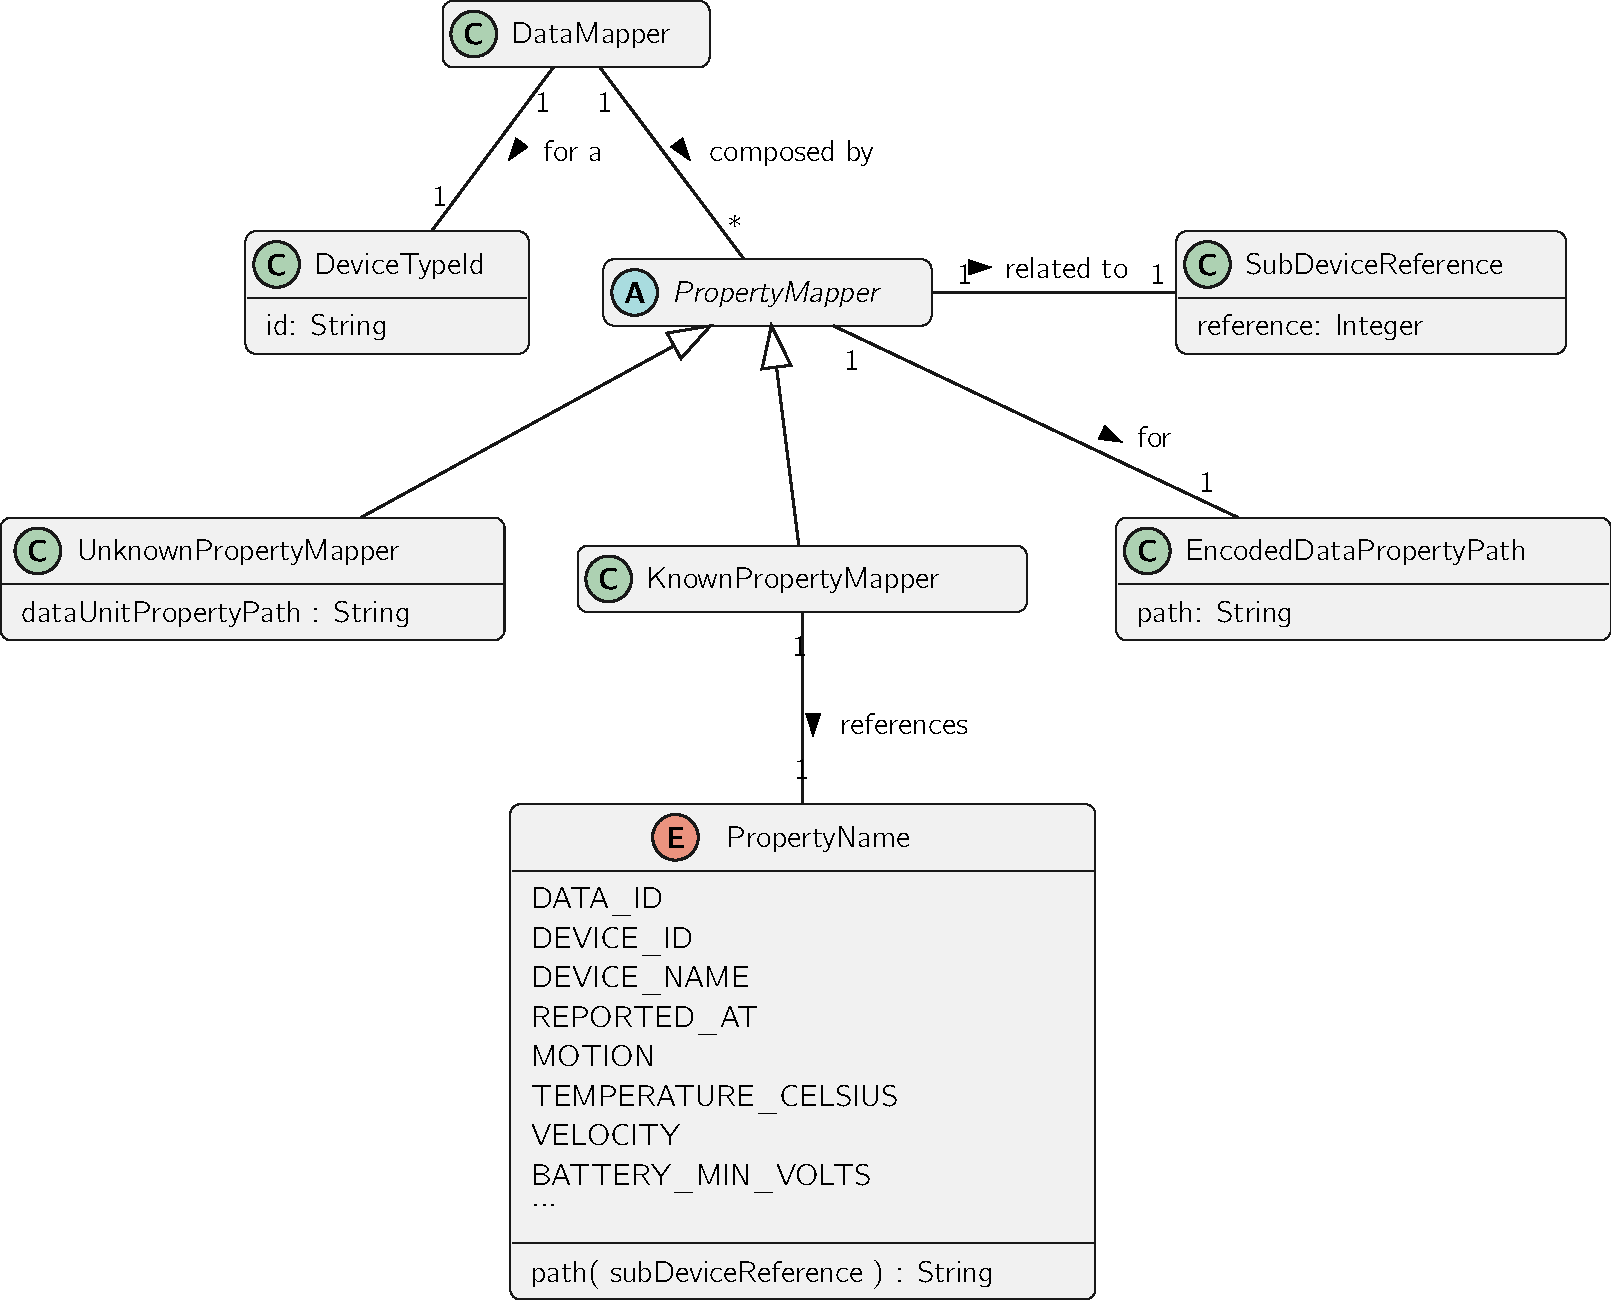
\includegraphics[page=1,width=\columnwidth]{assets/diagrams/design/domain/data-processor-model.pdf}
  \caption[Data Processor Concern Model]{Data Processor Concern Model}
  \label{fig:design:domain:bounded_contexts:processor:diagram}
\end{figure}

As a brief description:

\begin{itemize}
   \item \textbf{DataMapper}, the root entity in this concern is identified by a \textbf{DeviceTypeId} and has various instructions to map properties from the inbound information to a \textbf{Data Unit} properties;
   \item \textbf{DeviceTypeId} identifies the type of device that can be processed by this data mapper. When a data unit's message is supplied to this concern the data mapper that has the \textbf{DeviceTypeId} equal to the message's \textit{Device Type Options} routing key (mentioned in Table~\ref{tab:design:domain:shared_model:routing}) is used to process that data unit;
   \item \textbf{SubDeviceReference} represents a number that will be used later to reference a sub device when dealing with \textbf{Controller}s. For simple \textbf{Devices} the used and default value is \textit{0};
   \item \textbf{PropertyName} has much more properties that haven't been presented for brevity.
\end{itemize}

As an example, consider the inbound information represented as a JSON document with the structure in the example \ref{code:design:domain:bounded_contexts:processor:json}. To map the \textit{temperature} value to the \textbf{TEMPERATURE\_CELSIUS} property of a \textbf{Data Unit}, the \textbf{EncodedDataPropertyPath} would be \textit{decoded.data[0].temperature}.

\begin{lstlisting}[caption=Inbound Information Example, label={code:design:domain:bounded_contexts:processor:json}]
{
   "uuid": "de1a9d15-c018-4547-8453-87111cb4f81b",
   "id": "d81e6e69-1955-48a1-a1dd-4c812c15ebac",
   "time": 1657646955748,
   "decoded": {
      "data": [
         {
            "temperature": 18,
         }
      ]
   }
}
\end{lstlisting}

This process is simple since it expects the inbound information to be predisposed, but when working with \gls{IoT} Devices, to optimize the bandwidth used, it is common to send information encoded. The following section presents an alternative to this process.

\section{Data Decoder}
\label{subsubsec:design:domain:bounded_contexts:decoder}

The \textbf{Data Decoder} concern refers to a more complex data mapper that translates inbound information to \textbf{Data Unit}s, discussed in Section~\ref{subsubsec:design:domain:shared_model:data}.
It was created to deal with the limitations mentioned in Section~\ref{subsubsec:design:domain:bounded_contexts:processor}.

The received information is usually \textit{encoded}, meaning that the inbound information is received as it was sent by the \textbf{Device}, commonly as a \textit{Base64} encoded string, that needs to be processed so that information can be extracted.

The diagram in Figure~\ref{fig:design:domain:bounded_contexts:decoder:diagram} displays the noteworthy concepts in this concern.

\begin{figure}[H]
   \centering
  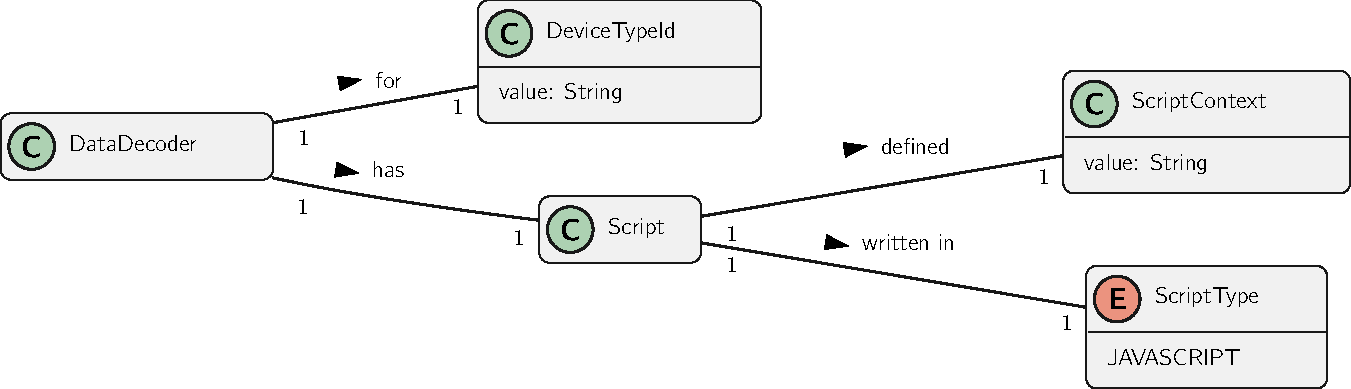
\includegraphics[page=1,width=\columnwidth]{assets/diagrams/design/domain/data-decoder-model.pdf}
  \caption[Data Decoder Concern Model]{Data Decoder Concern Model}
  \label{fig:design:domain:bounded_contexts:decoder:diagram}
\end{figure}

As a brief description:

\begin{itemize}
   \item \textbf{DataDecoder}, the root entity in this concern is identified by a \textbf{DeviceTypeId} and has a \textbf{Script};
   \item Currently, a \textbf{Script} can only be written in \textit{JavaScript} but in the future more languages like \textit{Python} or \textit{Groovy} can be added;
   \item The \textbf{ScriptContent} contains the code that will run for each inbound information that matches the \textbf{DeviceTypeId}.
\end{itemize}

This process requires some knowledge of the \textit{Javascript} language but it's much more flexible than the \textbf{Data Processor} operation.

\section{Device Management}
\label{subsubsec:design:domain:bounded_contexts:device}

The \textbf{Device Management} concern refers to the inventory of all registered \textbf{Device}s in the \textbf{Sensae Console}.

The diagram in Figure~\ref{fig:design:domain:bounded_contexts:device:diagram} displays the noteworthy concepts in this concern.

\begin{figure}[H]
   \centering
  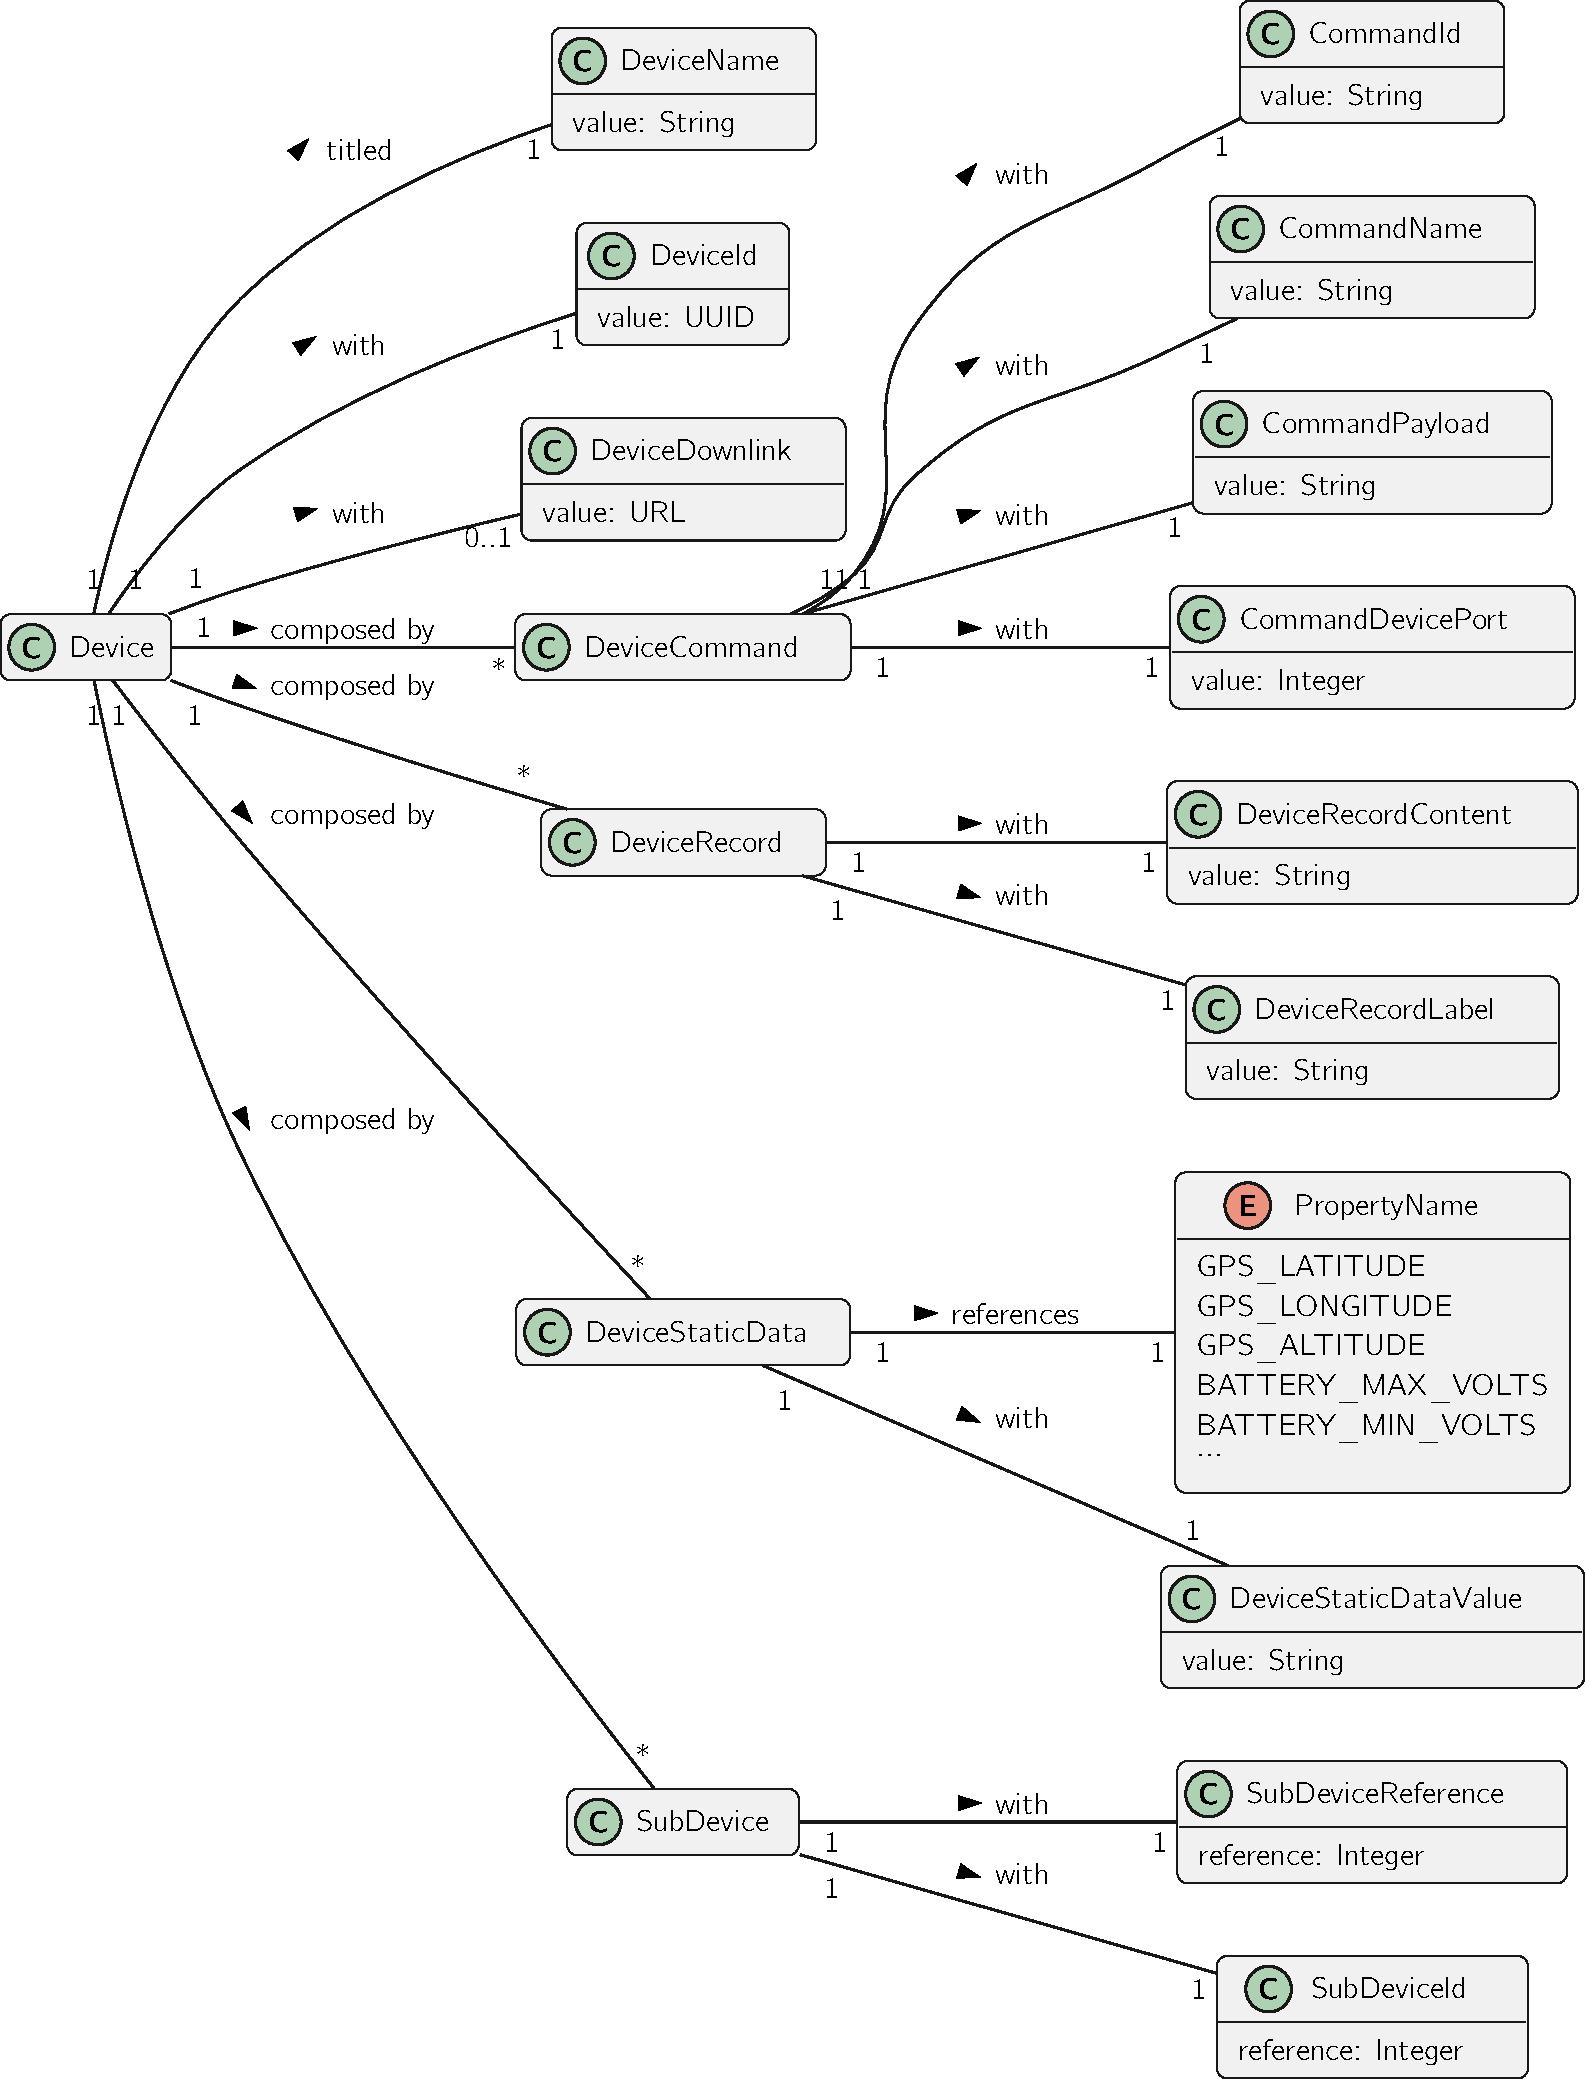
\includegraphics[page=1,width=\columnwidth]{assets/diagrams/design/domain/device-management-model.pdf}
  \caption[Device Management Concern Model]{Device Management Concern Model}
  \label{fig:design:domain:bounded_contexts:device:diagram}
\end{figure}

As a brief description:

\begin{itemize}
   \item A \textbf{Device} is uniquely identified by a \textbf{DeviceId} and a \textbf{DeviceName}. It may have a \textbf{DeviceDownlink}, an URL used to send device commands to;
   \item A \textbf{DeviceCommand} defines how to send a \textbf{Downlink} with a specific action;
   \item A \textbf{DeviceStaticData} helps to define data such as the device location;
   \item A \textbf{DeviceRecord} enriches the device information with anything deemed important. This can also help to group devices by projects, type of utility and others;
   \item A \textbf{SubDevice} references another \textbf{Device} by its \textbf{DeviceId}. This, coupled with the concepts \textbf{SubDeviceMeasures} and \textbf{SubDeviceCommands} presented in Figure~\ref{fig:design:domain:shared_model:data:diagram} help to split a \textbf{Controller}'s \textbf{Data Unit} into various \textbf{Data Unit}, one for each referenced \textbf{SubDevice}.
\end{itemize}

\section{Identity Management}
\label{subsubsec:design:domain:bounded_contexts:identity}

The \textbf{Identity Management} is concerned with identifying \textbf{Tenant}s, defining their permissions and what \textbf{Device}s they own.
To simplify this, a forth concept is introduced: \textbf{Domain}.

The diagram in Figure~\ref{fig:design:domain:bounded_contexts:identity:diagram} displays the noteworthy concepts in this concern.

\begin{figure}[H]
   \centering
  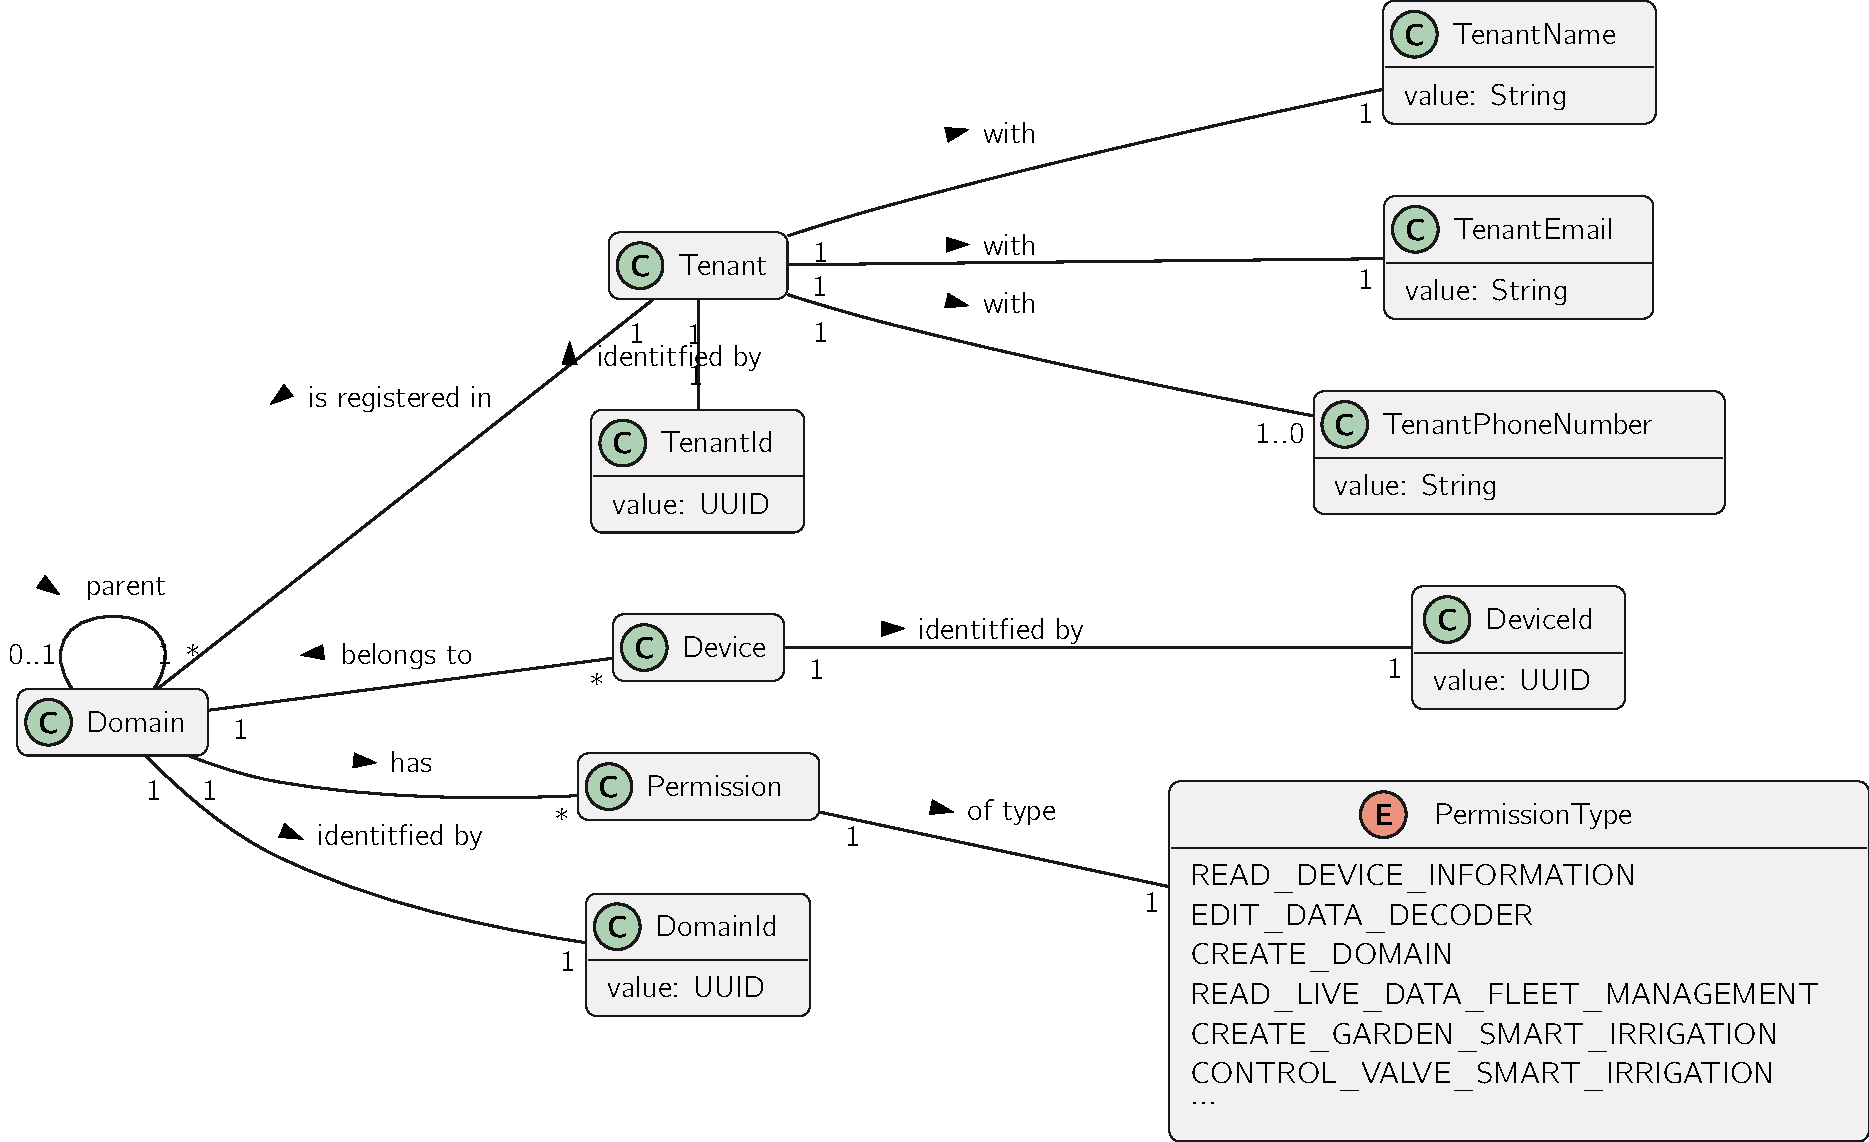
\includegraphics[page=1,width=\columnwidth]{assets/diagrams/design/domain/identity-management-model.pdf}
  \caption[Identity Management Concern Model]{Identity Management Concern Model}
  \label{fig:design:domain:bounded_contexts:identity:diagram}
\end{figure}

As a brief description:

\begin{itemize}
   \item A \textbf{Domain} is uniquely identified by a \textbf{DomainId} and can have a parent \textbf{Domain};
   \item There's a root \textbf{Domain}, the only one that doesn't have a parent and has all the available permissions;
   \item A \textbf{Tenant} has a \textbf{TenantName} and \textbf{TenantEmail}, unique \textbf{TenantId} and can have a \textbf{TenantPhoneNumber};
   \item A special \textbf{Tenant}, Anonymous, exists by default to give access to users without an account in the platform;
   \item A \textbf{Device} is uniquely identified by a \textbf{DeviceId};
   \item The \textbf{PermissionType} has much more types that haven't been presented for brevity.
\end{itemize}

A \textbf{Domain} represents a department in a hierarchical organization. An organization is composed by several domains in a tree like structure as presented in Figure~\ref{fig:design:domain:bounded_contexts:identity:organization}.

\begin{figure}[H]
   \centering
   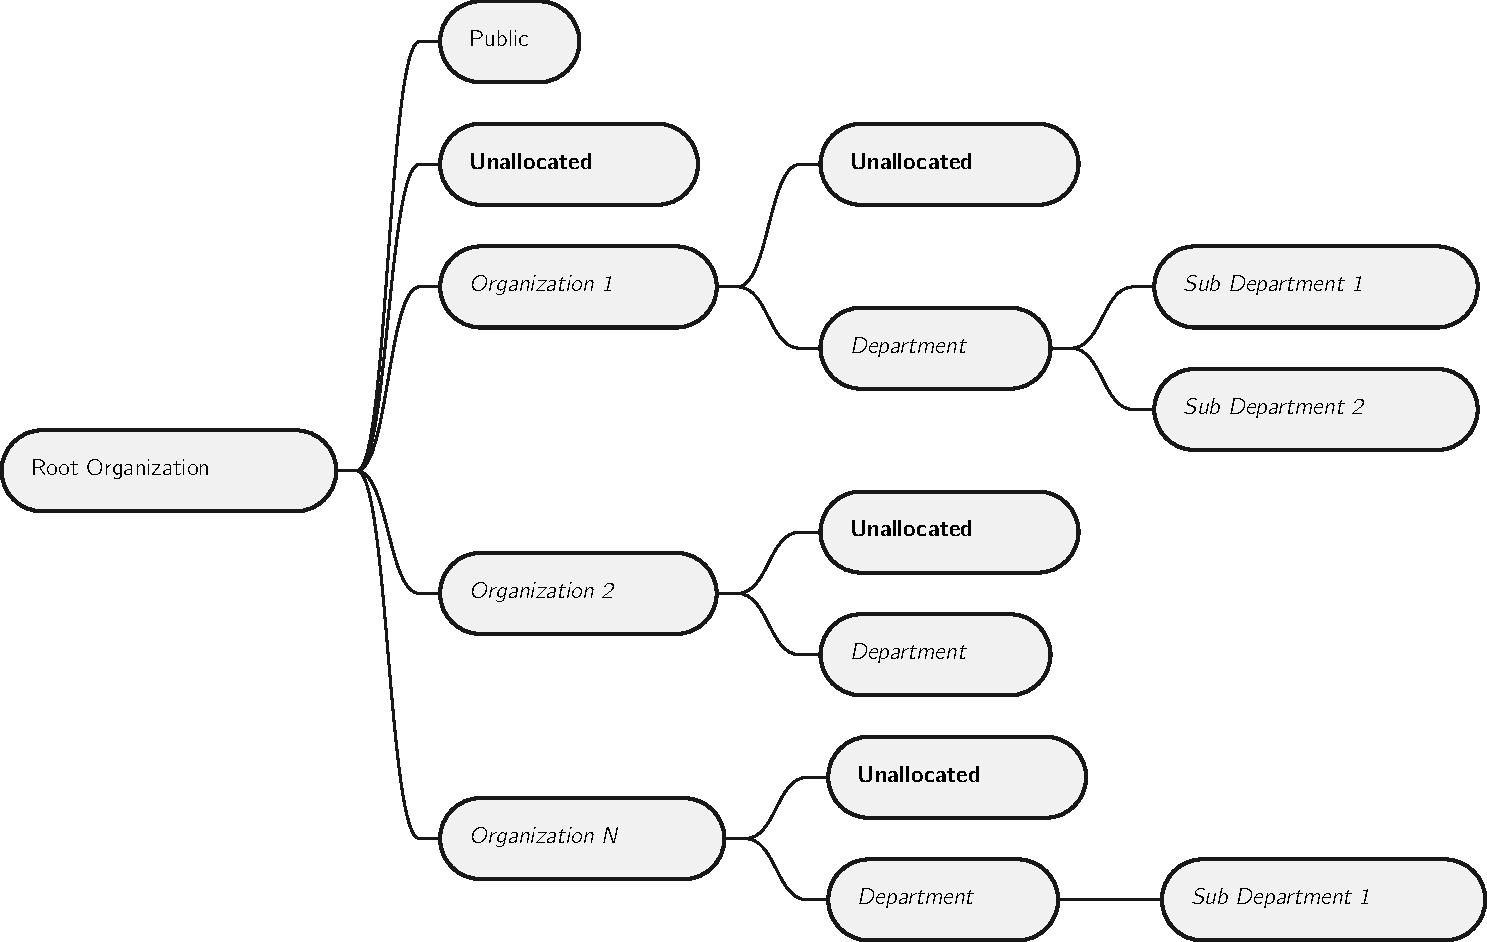
\includegraphics[page=1,width=\columnwidth]{assets/diagrams/design/domain/organization.pdf}
  \caption[Domain Structure]{Domain Structure}
  \label{fig:design:domain:bounded_contexts:identity:organization}
\end{figure}

Coupled with the figure above, there are other constrains:

\begin{itemize}
   \item A domain owns all devices in it and in his subdomains;
   \item A domain can only inherit his parent domain permissions;
   \item A tenant has all the domain permissions that he/she is registered in;
   \item A tenant can only see the devices that the domains he/she is registered in has access to;
   \item All \textit{Unallocated} domains have no permissions or devices and contain only tenants that are waiting to be assigned to a department or organization;
   \item The creation of an \textit{Organization} (level 2 domain), triggers the creation of its \textit{Unallocated} domain;
   \item The \textit{Public} domain can be accessed by any tenant, including those who are not authenticated in the system - with the Anonymous User account.
\end{itemize}

By default this concern contains the \textit{Root Organization} domain, the \textit{Root Organization}'s  \textit{Unallocated} domain and the \textit{Public} domain.

Referring to the roles in Section~\ref{subsec:requirements:functional:roles}, a Manager belongs to the \textit{Root Organization}, any Costumer belongs to one or various \textit{Organization}s, and the Anonymous user belongs to the \textit{Public} domain.
Ultimately, what defines a user role is the domain he/she belongs to. Even if an \textit{Organization} ends up having all available permissions it will not be able to control or access other \textit{Organization}'s device data or employees information.

\section{Rule Management}
\label{subsubsec:design:domain:bounded_contexts:rule}

The \textbf{Rule Management} concern refers to rule scenarios.

The purpose of this concern is to provide a high-level language that can analyze a stream of \textbf{Data Unit}s, identify abnormal occurrences, and output \textbf{Alert}s base on them.

In this concern, and according to Figure~\ref{fig:stateofart:arch:infra:rule:ifp} in Section~\ref{subsubsec:stateofart:arch:infra:rule}, the input data are \textbf{Data Unit}s and the output data are the \textbf{Alert}s. This concern is involved on how \textit{rules} are defined. The diagram in Figure~\ref{fig:design:domain:bounded_contexts:rule:diagram} displays the noteworthy concepts.

\begin{figure}[H]
   \centering
   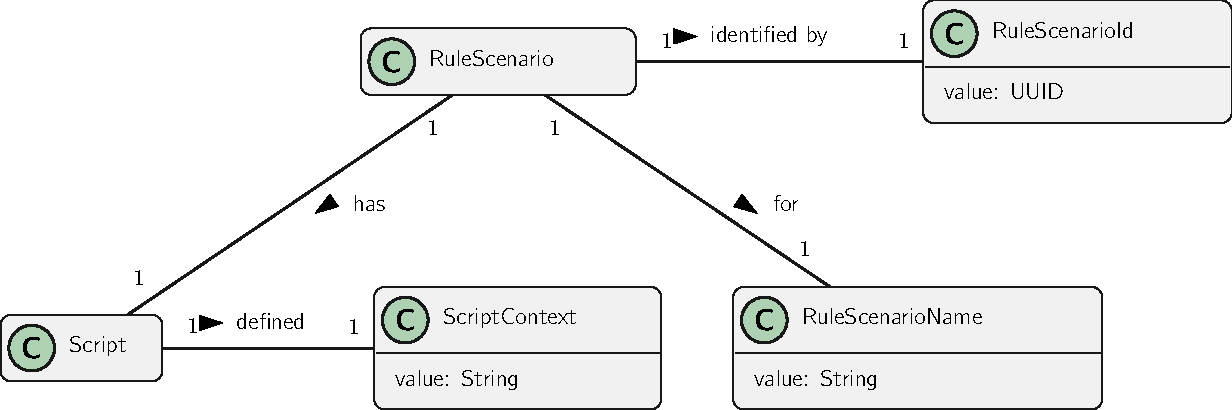
\includegraphics[page=1,width=\columnwidth]{assets/diagrams/design/domain/rule-management-model.pdf}
  \caption[Rule Management Concern Model]{Rule Management Concern Model}
  \label{fig:design:domain:bounded_contexts:rule:diagram}
\end{figure}
